\documentclass[aspectratio=169,11pt]{beamer}
\usepackage[T1]{fontenc}
\usepackage{lmodern,booktabs,array,tikz,pgfplots}
\pgfplotsset{compat=1.18}
\definecolor{Ink}{HTML}{17324D}
\definecolor{Teal}{HTML}{007F7B}
\definecolor{Gray}{HTML}{657483}
\definecolor{Rust}{HTML}{B5533C}
\setbeamercolor{alerted text}{fg=Rust}
\definecolor{Soft}{HTML}{EEF3F6}
\setbeamercolor{normal text}{fg=Ink,bg=white}
\setbeamercolor{frametitle}{fg=Ink}
\setbeamercolor{structure}{fg=Teal}
\setbeamercolor{block title}{fg=white,bg=Teal}
\setbeamercolor{block body}{fg=Ink,bg=Soft}
\setbeamertemplate{navigation symbols}{}
\setbeamersize{text margin left=9mm,text margin right=9mm}
\setbeamerfont{frametitle}{size=\large,series=\bfseries}
\setbeamertemplate{footline}{\hspace{9mm}\scriptsize From RL reproduction to RLM research | 14 Oct 2026, revised 20 Oct\hfill\insertframenumber/\inserttotalframenumber\hspace{9mm}\vspace{3mm}}
\newcommand{\source}[1]{\vfill{\scriptsize\color{Gray}#1\par}}
\hypersetup{pdftitle={A stronger foundation for RL on recursive language models},pdfauthor={Alex Towell}}
\title{A stronger foundation for RL on recursive language models}
\subtitle{Reproducing Segment Policy Optimization on GSM8K before extending RL to RLMs}
\author{Alex Towell}
\date{Advisor meeting, 14 October 2026 (revised 20 October)}
\begin{document}

\begin{frame}[plain]
\titlepage
\vfill
\begin{block}{In one sentence}
Rerunning the authors' SPO code on one A100 took the matched starting model from 39.8\% to
58.2\% on GSM8K (paper: 56.7\%) at an endpoint fixed before training; the RL workflow is now a
tested reference for the RLM work.
\end{block}
\end{frame}

\begin{frame}[t]
\frametitle{Before extending RL, establish that we can make it work.}
\textbf{The advisor's challenge:} reproduce a published learning result before
drawing conclusions from our more complex RLM experiments.
\medskip
\begin{block}{Why this matters}
Reinforcement learning (RL) trains a model using feedback on its own attempts.
We need evidence that our training and evaluation workflow can produce real improvement.
\end{block}
\medskip
\begin{columns}[T,onlytextwidth]
\begin{column}{.30\textwidth}
\textbf{Our starting question}\\[2mm]
Can feedback teach a model to use tools and delegate useful subtasks?
\end{column}
\begin{column}{.30\textwidth}
\textbf{The calibration exercise}\\[2mm]
Reproduce a known math RL result, where answers and the target score can be checked.
\end{column}
\begin{column}{.30\textwidth}
\textbf{What this buys us}\\[2mm]
A tested reference workflow for separating learning problems from measurement problems.
\end{column}
\end{columns}
\source{RLM = recursive language model: a model that can use code and call models on subtasks. The reproduction tests the RL workflow, not RLM performance.}
\end{frame}

\begin{frame}[t]
\frametitle{We reproduced the learning stage, not just a released model.}
\textbf{Experiment:} Segment Policy Optimization (SPO), a published RL method.\\
\textbf{Model and task:} RhoMath 1.1B on GSM8K arithmetic word problems; one A100.
\medskip
\begin{center}
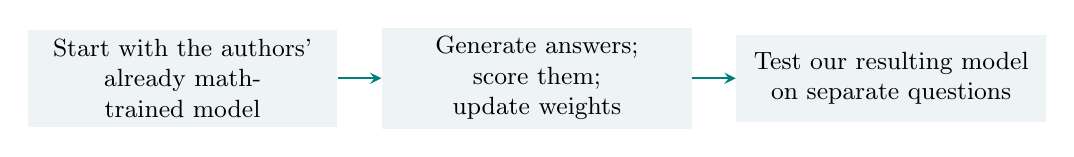
\begin{tikzpicture}[every node/.style={font=\small,align=center},>=stealth]
\node[fill=Soft,text width=3.7cm,minimum height=1.1cm] (a) at (0,0) {Start with the authors'\\already math-trained model};
\node[fill=Soft,text width=3.7cm,minimum height=1.1cm] (b) at (4.5,0) {Generate answers;\\score them;\\update weights};
\node[fill=Soft,text width=3.7cm,minimum height=1.1cm] (c) at (9,0) {Test our resulting model\\on separate questions};
\draw[->,thick,Teal] (a)--(b);
\draw[->,thick,Teal] (b)--(c);
\end{tikzpicture}
\end{center}
\begin{block}{What is distinctive about SPO?}
It samples possible continuations from parts of an answer to estimate which
parts increase the chance of success. This gives more local feedback than a final right/wrong label alone.
\end{block}
\textbf{Two different checks:} scoring the authors' trained model checks our
evaluator; training our own model tests whether we can reproduce learning.
\source{Guo et al., Segment Policy Optimization, arXiv:2505.23564v2, Sections 3--6 and Appendix H. We reproduce RL, not pretraining or the earlier supervised learning stage.}
\end{frame}

\begin{frame}[t]
\frametitle{Our own training recovered the paper's performance level.}
\begin{columns}[T,onlytextwidth]
\begin{column}{.61\textwidth}
\begin{tikzpicture}
\begin{axis}[width=\linewidth,height=4.9cm,xmin=0,xmax=11600,ymin=35,ymax=65,
xlabel={Training updates},ylabel={Correct sampled answers (\%)},
scaled x ticks=false,xtick={0,4000,8000,11040},xticklabels={0,4k,8k,11k},
ytick={35,40,45,50,55,60,65},tick label style={font=\scriptsize},
label style={font=\small},grid=major,grid style={gray!15},
legend style={font=\scriptsize,at={(.03,.97)},anchor=north west,draw=none,fill=white}]
\addplot[Teal,thick] table[x=updates,y=test_percent,col sep=comma]{learning-curve.csv};
\addlegendentry{Our training}
\addplot[Gray,dashed,thick] coordinates {(0,56.7)(11600,56.7)};
\addlegendentry{Paper: 56.7\%}
\addplot[only marks,mark=*,mark size=2.8pt,Teal] coordinates {(11040,58.1927596664)};
\end{axis}
\end{tikzpicture}
\end{column}
\begin{column}{.35\textwidth}
\small
\begin{tabular}{@{}lr@{}}
Matched start & 39.77\%\\
Paper target & 56.70\%\\
\textbf{Our final} & \textbf{58.19\%}\\
Best intermediate & 58.32\%\\
\end{tabular}
\medskip

\textbf{+18.42 percentage points}\\
over our starting model.
\medskip

12,281 correct / 21,104 answers.\\
1,319 questions, 16 answers each.
\medskip

\textbf{Fixed endpoint:}\\
11,040 updates. Not selected for the best score.
\end{column}
\end{columns}
\source{Metric: mean sampled-answer correctness (mean pass@1), not at-least-one-correct. Every scheduled test is shown; final answers independently regraded. One training seed; disclosed adaptations, not exact historical replay. Sources: final audit and curve provenance in evidence.md.}
\end{frame}

\begin{frame}[t]
\frametitle{The first attempt collapsed; the diagnosis is the main lesson.}
\small
\begin{columns}[T,onlytextwidth]
\begin{column}{.50\textwidth}
\textbf{What happened.} Test accuracy rose to 50.5\% at 4,336 updates, fell to
\alert{22.2\%} at 7,856, and the process crashed.
\medskip

\textbf{What we found.} An independent regrade showed the decline was real. Generation
requests began with the BOS token while training-side tokenization omitted it, so answers
were sampled under one input and scored under another. The crash: a batch guard zeroed four
batches in a row and the optimizer rejected the zero gradient.
\medskip

\textbf{What we did.} Three isolated, hash-pinned fixes; a restart from the original
weights; the endpoint fixed in advance.
\end{column}
\begin{column}{.46\textwidth}
\begin{block}{Lessons we carry forward}
\begin{itemize}\setlength{\itemsep}{1pt}
\item Score a known model first: it separates evaluator bugs from training bugs.
\item Report the gain from a matched start under one scoring rule.
\item Check that rewarded tokens are the scored tokens, BOS included.
\item Regrade saved answers independently; preserve failed runs.
\end{itemize}
\end{block}
\textbf{Answer to the advisor's challenge:} we can reproduce a published LLM RL result and
verify the gain. RLM is the next test.
\end{column}
\end{columns}
\source{docs/diagnosis-and-restart-20261012.md and evidence.md. The BOS mismatch is a supported hypothesis, not a demonstrated cause.}
\end{frame}

\begin{frame}[t]
\frametitle{Carry the discipline into RLM; test the new assumptions.}
\textbf{The new challenge:} an RLM must choose useful tool calls and subtasks,
combine their results, and do so within a limited budget.
\medskip
\begin{tabular}{@{}>{\raggedright\arraybackslash}p{.34\textwidth}>{\raggedright\arraybackslash}p{.59\textwidth}@{}}
\toprule
Question for RLM & Small next comparison \textit{(proposed, not yet a result)}\\
\midrule
Can the starting model use the workflow? &
Direct answers versus RLM before RL, on the same tasks:
check tool use, correctness and cost.\\[2mm]
Does RL improve useful decisions? &
The same RLM before versus after RL:
untouched evaluation tasks, matched budgets.\\[2mm]
Would more local feedback help? &
After a basic learning signal: final-outcome rewards
versus feedback on intermediate decisions.\\
\bottomrule
\end{tabular}
\medskip
\textbf{Keep:} checked rewards, matched baselines, fixed evaluation rules, saved evidence.\\
\textbf{Do not assume:} SPO or its exact settings will transfer to RLM.
\source{We now have a credible RL reference point. Next: test learning in a recursive, tool-using environment. These comparisons are proposals, not completed RLM results.}
\end{frame}

\appendix
\begin{frame}[t]
\frametitle{Appendix: what exactly was reproduced and checked?}
\small
\begin{tabular}{@{}>{\raggedright\arraybackslash}p{.25\textwidth}>{\raggedright\arraybackslash}p{.68\textwidth}@{}}
\toprule
Item & Recorded protocol or limitation\\
\midrule
Training &
Authors' RhoMath 1.1B starting weights; SPO-chain interval 5; seed 42;
690 collections / 11,040 updates, original 1,000-collection learning-rate horizon.\\[2mm]
Data and test &
7,100 training / 373 validation / 1,319 test questions.
16 test samples per question; temperature 0.35; effective top-p 1.0.\\[2mm]
Independent checks &
All 33,024 final answers across three splits and 21 metrics rechecked.
Final full model/optimizer checkpoint preserved with matching file hashes.\\[2mm]
Reference checks &
Authors' released model: 56.69\%, versus paper 56.7\%.
Our starting model: 39.77\%, versus paper starting reference 40.3\%.\\[2mm]
Fidelity and scope &
Process-local BOS token alignment and BF16 numerical adapters disclosed.
Historical equivalence unresolved. One seed; no causal
ablation or measured RLM transfer.\\
\bottomrule
\end{tabular}
\source{BOS = beginning-of-sequence token; BF16 = numerical format used in training. Full protocol, immutable audit references and implementation disclosures: evidence.md and the linked final research report.}
\end{frame}
\end{document}
